\documentclass[10pt,a4paper]{article}
\usepackage[utf8]{inputenc}

% \usepackage{ngerman}  % german documents
\usepackage{graphicx}  % import graphics einbinden
\usepackage{listings}  % support source code listing
\usepackage{amsmath}  % math stuff
\usepackage{amssymb} % 
\usepackage{a4wide} % wide pages
\usepackage{fancyhdr} % nice headers
\usepackage{tikz} %graphs
\usetikzlibrary{arrows}
\lstset{basicstyle=\footnotesize,language=Python,numbers=left, numberstyle=\tiny, stepnumber=5,firstnumber=0, numbersep=5pt} % set up listings
\pagestyle{fancy}             % header
\setlength{\parindent}{0pt}   % no indentation

\usepackage[pdfpagemode=None, colorlinks=true,  % url coloring
           linkcolor=blue, urlcolor=blue, citecolor=blue, plainpages=false, 
           pdfpagelabels,unicode]{hyperref}
           
% change enums style: first level (a), (b), (c)           
\renewcommand{\labelenumi}{(\alph{enumi})}
\renewcommand{\labelenumii}{(\arabic{enumii})}

%lecture name
\newcommand{\lecture}{
	Bioinformatics III
}           

%assignment iteration
\newcommand{\assignment}{
	Third Assignment
}

%set up names, matricle number, and email
\newcommand{\authors}{
  \begin{tabular}{rl}
    \href{mailto:s9alfloh@stud.uni-saarland.de}{Alexander Flohr} & (2549738)\\
    \href{mailto:s9ankupi@stud.uni-saarland.de}{Andrea Kupitz} & (2550260)
  \end{tabular}
}

% use to start a new exercise
\newcommand{\exercise}[1]
{
  \stepcounter{subsection}
  \subsection*{Exercise \thesubsection: #1}

}

\begin{document}
\title{\Large \lecture \\ \textbf{\normalsize \assignment}}
\author{\authors}

\setlength \headheight{25pt}
\fancyhead[R]{\begin{tabular}{r}\lecture \\ \assignment \end{tabular}}
\fancyhead[L]{\authors}


\setcounter{section}{3} % modify for later sheets, i.e. 2, 3, ...
%\section{Introduction to Python and some Network Properties} % optional, note that section invocation sets the section counter + 1, so adapt the setcounter command
\maketitle

\exercise{Naive Bayes classifier}
\begin{enumerate}
\item Because the features are independent: \begin{equation}P(S) = \prod_{i} P(S_i) \end{equation}
Following the Bayes theorem: \begin{equation} \frac{P(S|C) * P(C)} {P(S)} = P(C|S) \end{equation}
Further \begin{equation} log( \frac{P(C|S)} {P(\bar{C}|S)} ) = log( \prod_{i} \frac{ \frac{P(S_i|C) * P(C)}{P(S_i)} }{ \frac{P(S_i|\bar{C}) * P(\bar{C})}{P(S_i)} } ) = \sum_{i} log( \frac{P(S_i|C) * P(C)}{P(S_i|\bar{C}) * P(\bar{C})} ) \end{equation}
The actual classification is done by evaluating the sum over the log-likelihood ratios. If the sum is smaller zero, it means most of the log-likelihoods were smaller zero because the probability of $\bar{C}$ was greater than the one for C. Therefore, the state sequence evaluates to "no interaction". Vice versa, if the sum over the likelihoods was greater than zero, we classify 1, which means there is an interaction between the proteins.

\item The logarithm of the ratio enables to see directly if the probability is higher that the observed states belong to interacting or non-interacting proteins.
Moreover the ratio of the likelihoods normalizes the probabilities because states occurring more often will have the same ratio than less frequent ones.\\
This classification may perform bad on real-world data if a feature classifies all interactions to the same class because we cannot handle probabilities being zero. Moreover classification is bad if the dataset is small because the classification may be biased to one class.

\item Listing \ref{ex1-1} shows source code.
\lstinputlisting[label=ex1-1,caption={Example Listing of source code}] {model.py}
P(C) = 0.5125628140703518\\
P($\bar{C}$) = 0.48743718592964824\\
Table \ref{tab1} shows best 10 absolute features.\\
The 10 features in table \ref{tab1} seem to be the most promising features to recognize protein interactions correctly because their log-likelihood is very high. There is no specific region of features which seems to be very helpful. The best ten features are rather widely spread. Further, no state variant seems to indicate an interaction.
\begin{table}[!h]
\label{tab1}
\begin{tabular}{llll}
enumeration of best features & log ratio & feature number & state variant\\
\hline
1 & -1.896088525279219 & 33 & 0\\
2 & 1.2025011337144798 & 25 & 2\\
3 & 1.0175787952204678 & 33 & 2\\
4 & 0.7074238669166282 & 33 & 1\\
5 & 0.642885345779057 & 40 & 2\\
6 & -0.6380484996830071 & 57 & 2\\
7 & 0.6003257313602611 & 81 & 0\\
8 & -0.5271859068711975 & 95 & 2\\
9 & -0.4885167657120435 & 88 & 0\\
10 & -0.4885167657120435 & 89 & 1\\
\end{tabular}
\caption{best 10 features}
\end{table}

\item Listing \ref{ex1-1} shows source code.\\
The classification is equally distributed between both classes. But the accuracy is rather low.\\
For "test1.tsv" the classification is: [1, 1, 1, 1, 1, 1, 0, 1, 1, 0, 1, 0, 1, 1, 0, 1, 1, 1, 1, 1, 1, 1, 1, 1, 0, 0, 1, 1, 0, 0, 0, 1, 1, 1, 1, 1, 0, 1, 1, 1, 1, 0, 1, 0, 1, 1, 1, 1, 0, 1, 1, 1, 1, 0, 0, 1, 0, 0, 1, 0, 1, 1, 1, 0, 0, 1, 1, 1, 1, 1, 0, 1, 0, 0, 1, 1, 1, 1, 0, 0, 1, 1, 1, 1, 1, 0, 0, 1, 0, 1, 1, 0, 0, 1, 0, 0, 0, 1, 0, 1]\\
Whereby each position in the list corresponds to the protein pair in the test file at the same position. The exact value of the accuracy is 0.5757575757575758.

\item P(C) = 0.7839195979899497\\
P($\bar{C}$) = 0.2160804020100503\\
Table \ref{tab2} shows best 10 features.\\
\begin{table}[!h]
\label{tab2}
\begin{tabular}{llll}
enumeration of best features & log ratio & feature number & state variant\\
\hline
1 & -1.9818030721159199 & 33 & 0\\
2 & 1.2762934659055623 & 83 & 0\\
3 & 0.9886113934537812 & 99 & 0\\
4 & 0.9085686857802447 & 98 & 3\\
5 & 0.8514102719402962 & 99 & 3\\
6 & -0.7290401036205519 & 87 & 1\\
7 & 0.7166776779701394 & 74 & 0\\
8 & 0.7037742731342315 & 90 & 1\\
9 & 0.6774569648168581 & 91 & 1\\
10 & 0.6155815610987706 & 63 & 0\\
\end{tabular}
\caption{best 10 features}
\end{table}
\end{enumerate}
For "test2.tsv" the classification is: [0, 0, 1, 1, 1, 0, 1, 0, 0, 0, 1, 0, 0, 1, 0, 0, 0, 0, 1, 1, 0, 1, 1, 0, 0, 0, 0, 0, 1, 1, 0, 0, 0, 0, 0, 0, 0, 0, 0, 1, 0, 0, 1, 0, 0, 1, 1, 1, 0, 0, 0, 1, 0, 1, 0, 0, 0, 1, 0, 0, 1, 0, 0, 1, 0, 0, 0, 0, 1, 1, 0, 1, 0, 0, 1, 1, 0, 0, 0, 0, 0, 1, 0, 1, 0, 0, 1, 1, 1, 1, 0, 1, 1, 1, 0, 0, 1, 1, 1, 0]\\
The accuracy is 0.37373737373737376.\\
The classification might be worse for the second test set because in the second trainings set, interacting proteins occur more often than non-interacting ones which may lead to proteins rather been interpreted as interacting.
\newpage
\exercise{Network communities}
\begin{enumerate}
\item The maximal finite value that the edge-clustering coefficient can take is 2 because it is maximal if the numerator is maximal and the denominator is minimal. The denominator cannot get smaller than 0 because every pair of nodes will have at least one edge between them. Because division by zero is undefined, we take the next value 1, which means that the nodes both have at least one more edge than the one to each other. If both nodes have at least two edges, there is maximal one triangle between them if they are connected to the same node. Therefore, the numerator is 2. If there were more triangles between the nodes, the denominator would also increase and the ratio is smaller. Thus, 2 is the maximal value the coefficient can take. Figure \ref{fig2_1} shows an example of a network with maximal clustering coefficient between all nodes.\\
\newline
\begin{figure}
\begin{center}
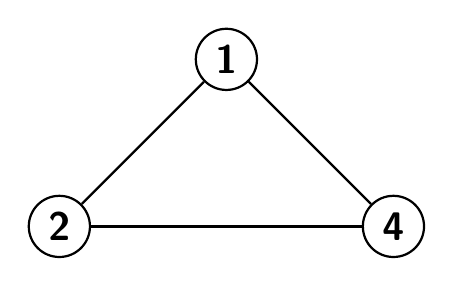
\begin{tikzpicture}[auto, node distance=3cm, every loop/.style={},
                    thick,main node/.style={circle,draw,font=\sffamily\Large\bfseries}]
  \label{fig2_1}
  \node[main node] (1) {1};
  \node[main node] (2) [below left of=1] {2};
  \node[main node] (4) [below right of=1] {4};
  \path[every node/.style={font=\sffamily\small}]
    (1) edge node [left] {} (4)
    (2) edge node [right] {} (1)
        edge node {} (4);
\end{tikzpicture}
\caption{example of network with maximal clustering coefficient}
\end{center}
\end{figure}

\item
\begin{enumerate}
\item Listing \ref{ex2-2} shows source code.
\lstinputlisting[label=ex2-2,caption={Example Listing of source code}] {DecompositionNetwork.py}
Resulting detetion order:\\
\texttt{
Remove edge with clustering coefficient 0.0 :	 Baelish - Varys\\
Remove edge with clustering coefficient 0.0 :	 Tyrion - Shae\\
Remove edge with clustering coefficient 0.5 :	 Hound - Joffrey\\
Remove edge with clustering coefficient 0.5 :	 Jon - Eddard\\
Remove edge with clustering coefficient 0.5 :	 Eddard - Robert\\
Remove edge with clustering coefficient 0.5 :	 Sansa - Tyrion\\
Remove edge with clustering coefficient 1.0 :	 Hound - Mountain\\
Remove edge with clustering coefficient 0.0 :	 Hound - Arya\\
Remove edge with clustering coefficient 0.0 :	 Mountain - Cersei\\
Remove edge with clustering coefficient 1.0 :	 Joffrey - Jaime\\
Remove edge with clustering coefficient $1.\bar{3}$ :	 Catelyn - Sansa\\
Remove edge with clustering coefficient 1.0 :	 Arya - Catelyn\\
Remove edge with clustering coefficient 1.0 :	 Eddard - Catelyn\\
Remove edge with clustering coefficient 0.0 :	 Catelyn - Baelish\\
Remove edge with clustering coefficient 0.0 :	 Sansa - Baelish\\
Remove edge with clustering coefficient 2.0 :	 Joffrey - Cersei\\
Remove edge with clustering coefficient 0.0 :	 Joffrey - Robert\\
Remove edge with clustering coefficient 0.0 :	 Cersei - Robert\\
Remove edge with clustering coefficient 2.0 :	 Arya - Eddard\\
Remove edge with clustering coefficient 0.0 :	 Arya - Sansa\\
Remove edge with clustering coefficient 0.0 :	 Eddard - Sansa\\
Remove edge with clustering coefficient 2.0 :	 Cersei - Jaime\\
Remove edge with clustering coefficient 0.0 :	 Cersei - Tyrion\\
Remove edge with clustering coefficient 0.0 :	 Jaime - Tyrion\\
Remove edge with clustering coefficient 2.0 :	 Jeor - Samwell\\
Remove edge with clustering coefficient 0.0 :	 Jeor - Jon\\
Remove edge with clustering coefficient 0.0 :	 Samwell - Jon}

\newpage
\item Figure \ref{fig2_2} shows the dendrogram of the network.
\begin{figure}
\begin{center}
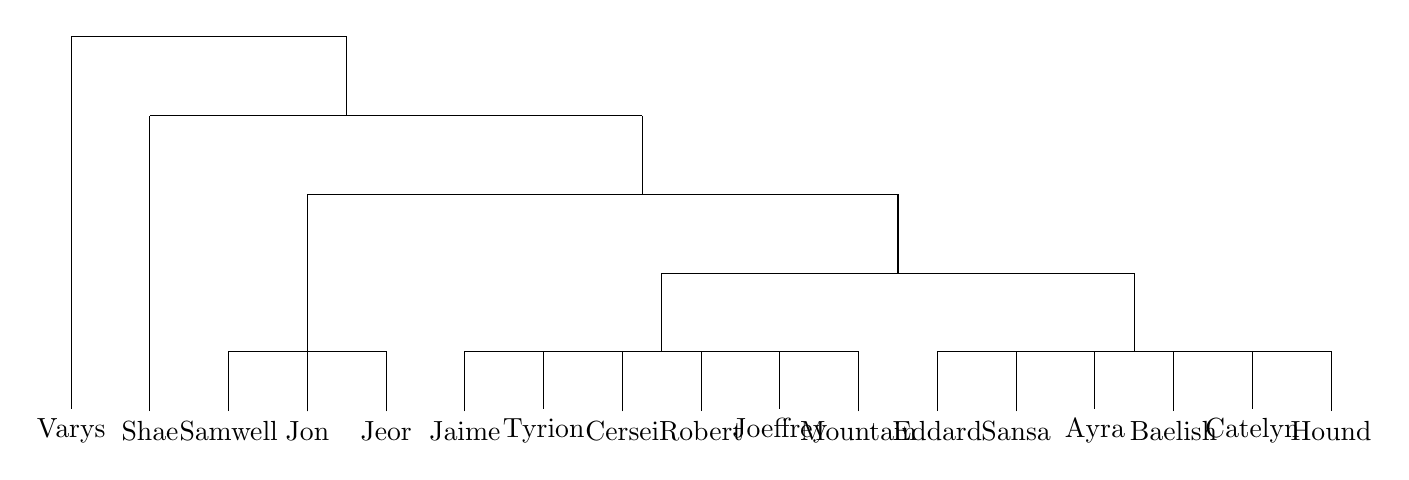
\begin{tikzpicture}[sloped]
\label{fig2_2}
\node (a) at (-15,0) {Samwell};
\node (b) at (-14,0) {Jon};
\node (c) at (-13,0) {Jeor};
\node (d) at (-12,0) {Jaime};
\node (e) at (-11,0) {Tyrion};
\node (f) at (-10,0) {Cersei};
\node (g) at (-6,0) {Eddard};
\node (h) at (-5,0) {Sansa};
\node (i) at (-4,0) {Ayra};
\node (j) at (-9,0) {Robert};
\node (k) at (-8,0) {Joeffrey};
\node (l) at (-3,0) {Baelish};
\node (m) at (-2,0) {Catelyn};
\node (n) at (-7,0) {Mountain};
\node (o) at (-1,0) {Hound};
\node (p) at (-17,0) {Varys};
\node (q) at (-16,0) {Shae};
\node (ab) at (-14.5,1) {};
\node (bc) at (-14,1) {};
\node (de) at (-11.5,1) {};
\node (ef) at (-11,1) {};
\node (gh) at (-5.5,1) {};
\node (hi) at (-5,1) {};
\node (fj) at (-10,1) {};
\node (jk) at (-9,1) {};
\node (il) at (-4,1) {};
\node (lm) at (-3,1) {};
\node (kn) at (-8,1) {};
\node (mo) at (-2,1) {};
\node (dn) at (-9.5,2) {};
\node (go) at (-3.5,2) {};
\node (dnunten) at (-9.5,1) {};
\node (gounten) at (-3.5,1) {};
\node (ac) at (-14,3) {};
\node (do) at (-6.5,3) {};
\node (dounten) at (-6.5,2) {};
\node (Q) at (-16,4) {};
\node (ao) at (-9.75,4) {};
\node (aounten) at (-9.75,3) {};
\node (P) at (-17,5) {};
\node (aq) at (-13.5,5) {};
\node (aqunten) at (-13,4) {};
\draw  (a) |- (ab.center);
\draw  (b) |- (ab.center);
\draw  (c) |- (bc.center);
\draw  (d) |- (de.center);
\draw  (e) |- (de.center);
\draw  (f) |- (ef.center);
\draw  (g) |- (gh.center);
\draw  (h) |- (gh.center);
\draw  (i) |- (hi.center);
\draw  (j) |- (fj.center);
\draw  (k) |- (jk.center);
\draw  (l) |- (il.center);
\draw  (m) |- (lm.center);
\draw  (n) |- (kn.center);
\draw  (o) |- (mo.center);
\draw  (dn.center) |- (go.center);
\draw  (dnunten.center) |- (dn.center);
\draw  (gounten.center) |- (go.center);
\draw  (ac.center) |- (do.center);
\draw  (b) |- (ac.center);
\draw  (dounten.center) |- (do.center);
\draw  (Q) |- (ao.center);
\draw  (q) |- (Q);
\draw  (ao.center) |- (aounten.center);
\draw  (P) |- (aq.center);
\draw  (p) |- (P);
\draw  (aq.center) |- (aqunten.center);
\end{tikzpicture}
\caption{dendrogram of communities}
\end{center}
\end{figure}
\end{enumerate}

\item Figure \ref{fig-1} shows the visually determined two disjoint communities. For both communities the strong criterion applies. For all nodes besides Ayra, Eddard and Sansa from community one and the Hound, Robert and Tyrion from community two applies that they are only connected to nodes within the same community. Whereas the six outliers have one edge to the outside but at least two links to the inside, which means for every member of the subgraph V holds, it has more links to the inside of the community ($k^{in}$) than to the outside ($k^{out}$):\\
\begin{equation}
k^{in}_i (V) > k^{out}_i (V) \forall i \in V
\end{equation}
\begin{figure}
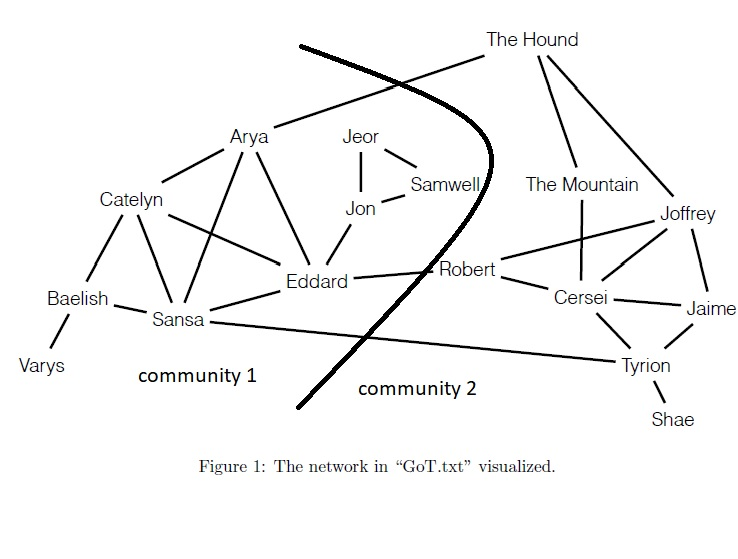
\includegraphics[scale=1]{task2c).jpg}
\caption{Visualization of two disjoint communities}
\label{fig-1}
\end{figure}
\end{enumerate}

\end{document}